%Version 3.1 December 2024
% See section 11 of the User Manual for version history
%%%%%%%%%%%%%%%%%%%%%%%%%%%%%%%%%%%%%%%%%%%%%%%%%%%%%%%%%%%%%%%%%%%%%%
%%                                                                 %%
%% Please do not use \input{...} to include other tex files.       %%
%% Submit your LaTeX manuscript as one .tex document.              %%
%%                                                                 %%
%% All additional figures and files should be attached             %%
%% separately and not embedded in the \TeX\ document itself.       %%
%%                                                                 %%
%%%%%%%%%%%%%%%%%%%%%%%%%%%%%%%%%%%%%%%%%%%%%%%%%%%%%%%%%%%%%%%%%%%%%
%%\documentclass[referee,sn-basic]{sn-jnl}% referee option is meant for double line spacing

%%=======================================================%%
%% to print line numbers in the margin use lineno option %%
%%=======================================================%%

%%\documentclass[lineno,pdflatex,sn-basic]{sn-jnl}% Basic Springer Nature Reference Style/Chemistry Reference Style

%%=========================================================================================%%
%% the documentclass is set to pdflatex as default. You can delete it if not appropriate.  %%
%%=========================================================================================%%

%%\documentclass[sn-basic]{sn-jnl}% Basic Springer Nature Reference Style/Chemistry Reference Style
%%Note: the following reference styles support Namedate and Numbered referencing. By default the style follows the most common style. To switch between the options you can add or remove �Numbered� in the optional parenthesis.
%%The option is available for: sn-basic.bst, sn-chicago.bst%

\documentclass[pdflatex,sn-nature,lineno]{sn-jnl}% Style for submissions to Nature Portfolio journals
%\documentclass[pdflatex,sn-basic]{sn-jnl}% Basic Springer Nature Reference Style/Chemistry Reference Style
%\documentclass[pdflatex,sn-mathphys-num]{sn-jnl}% Math and Physical Sciences Numbered Reference Style
%\documentclass[pdflatex,sn-mathphys-ay]{sn-jnl}% Math and Physical Sciences Author Year Reference Style
%\documentclass[pdflatex,sn-aps]{sn-jnl}% American Physical Society (APS) Reference Style
%\documentclass[pdflatex,sn-vancouver-num]{sn-jnl}% Vancouver Numbered Reference Style
%\documentclass[pdflatex,sn-vancouver-ay]{sn-jnl}% Vancouver Author Year Reference Style
%\documentclass[pdflatex,sn-apa]{sn-jnl}% APA Reference Style
%\documentclass[pdflatex,sn-chicago]{sn-jnl}% Chicago-based Humanities Reference Style

%%%% Standard Packages
%%<additional latex packages if required can be included here>
\usepackage{graphicx}%
\usepackage{multirow}%
\usepackage{amsmath,amssymb,amsfonts}%
\usepackage{amsthm}%
\usepackage{mathrsfs}%
\usepackage[title]{appendix}%
\usepackage{xcolor}%
\usepackage{textcomp}%

% Define argmax operator
\DeclareMathOperator*{\argmax}{argmax}
\usepackage{manyfoot}%
\usepackage{booktabs}%
\usepackage{algorithm}%
\usepackage{algorithmicx}%
\usepackage{algpseudocode}%
\usepackage{listings}%

% \usepackage{caption}
\usepackage{standalone}
\usepackage{tikz}
\usepackage[dvipsnames]{xcolor}
\usepackage{geometry}
\usepackage{textcomp} % using \textquotesingle
% Minted package for beautiful syntax highlighting
\usepackage{minted}
\usemintedstyle{borland}
\setminted{
  fontsize=\small,
  breaklines=true,
  autogobble,
  frame=single,
  framesep=2mm,
  linenos
}

% Use bash lexer for TSG code examples (since it handles # comments well)
\newminted{bash}{
  fontsize=\small,
  breaklines=true,
  autogobble,
  frame=single,
  framesep=2mm,
  linenos
}

\usetikzlibrary{shadows,shapes,arrows,positioning,fit,backgrounds,decorations.pathreplacing,calc}

\graphicspath{{../figures}}

\usepackage[acronym, automake, style=index, shortcuts]{glossaries-extra}
\setabbreviationstyle[acronym]{long-short}
% define glossaries
\makeglossaries

\newacronym{wga}{WGA}{Whole Genome Amplification}
\newacronym{mda}{MDA}{Multiple Displacement Amplification}
\newacronym{malbac}{MALBAC}{Multiple Annealing and Looping-based Amplification Cycles}
\newacronym{gpu}{GPU}{Graphics Processing Unit}
\newacronym{cpu}{CPU}{Central Processing Unit}
\newacronym{hpc}{HPC}{High Performance Computing}
\newacronym{sv}{SV}{Structural Variation}
\newacronym{snp}{SNP}{Single Nucleotide Polymorphism}
\newacronym{ont}{ONT}{Oxford Nanopore Technologies}
\newacronym{pb}{PacBio}{Pacific Biosciences}
\newacronym{del}{DEL}{deletion}
\newacronym{dup}{DUP}{duplication}
\newacronym{ins}{INS}{insertion}
\newacronym{inv}{INV}{inversion}
\newacronym{tra}{TRA}{translocation}
\newacronym{pcr}{PCR}{Polymerase Chain Reaction}
\newacronym{mrna}{mRNA}{messenger RNA}
\newacronym{facs}{FACS}{Fluorescence-activated cell sorting}
\newacronym{sa}{SA}{Supplementary Alignment}
\newacronym{lianti}{LIANTI}{Linear Amplification via Transposon Insertion}
\newacronym{doppcr}{DOP-PCR}{Degenerate Oligonucleotide-Primed PCR}
\newacronym{pta}{PTA}{Primary Template-directed Amplification}
\newacronym{dmda}{dMDA}{droplet-based MDA}

\newacronym{ide}{IDE}{Integrated Development Environment}
\newacronym{cd}{CD}{Continuous Development}
\newacronym{ucsc}{UCSC}{UCSC Genome Browser}

\newacronym{glm}{GLM}{Genomic Language Model}
\newacronym{lcglm}{LCGLM}{long-context genomic language model}
\newacronym{mlp}{MLP}{multilayer perceptron}
\newacronym{gelu}{GELU}{Gaussian Error Linear Unit}

%%%%%=============================================================================%%%%
%%%%  Remarks: This template is provided to aid authors with the preparation
%%%%  of original research articles intended for submission to journals published
%%%%  by Springer Nature. The guidance has been prepared in partnership with
%%%%  production teams to conform to Springer Nature technical requirements.
%%%%  Editorial and presentation requirements differ among journal portfolios and
%%%%  research disciplines. You may find sections in this template are irrelevant
%%%%  to your work and are empowered to omit any such section if allowed by the
%%%%  journal you intend to submit to. The submission guidelines and policies
%%%%  of the journal take precedence. A detailed User Manual is available in the
%%%%  template package for technical guidance.
%%%%%=============================================================================%%%%

%% as per the requirement new theorem styles can be included as shown below
\theoremstyle{thmstyleone}%
\newtheorem{theorem}{Theorem}%  meant for continuous numbers
%%\newtheorem{theorem}{Theorem}[section]% meant for sectionwise numbers
%% optional argument [theorem] produces theorem numbering sequence instead of independent numbers for Proposition
\newtheorem{proposition}[theorem]{Proposition}%
%%\newtheorem{proposition}{Proposition}% to get separate numbers for theorem and proposition etc.

\theoremstyle{thmstyletwo}%
\newtheorem{example}{Example}%
\newtheorem{remark}{Remark}%

\theoremstyle{thmstylethree}%
\newtheorem{definition}{Definition}%

\raggedbottom
%%\unnumbered% uncomment this for unnumbered level heads

\begin{document}

\title[Article Title]{ChimeraLM filters amplification artifacts for accurate structural variant calling in long-read single-cell sequencing}

%%=============================================================%%
%% GivenName	-> \fnm{Joergen W.}
%% Particle	-> \spfx{van der} -> surname prefix
%% FamilyName	-> \sur{Ploeg}
%% Suffix	-> \sfx{IV}
%% \author*[1,2]{\fnm{Joergen W.} \spfx{van der} \sur{Ploeg}
%%  \sfx{IV}}\email{iauthor@gmail.com}
%%=============================================================%%
\author[1]{\fnm{Yangyang} \sur{Li}}\email{yangyang.li@northwestern.edu}
\equalcont{These authors contributed equally to this work.}
\author[1]{\fnm{Qingxiang} \sur{Guo}}\email{qingxiang.guo@northwestern.edu}
\equalcont{These authors contributed equally to this work.}
\author*[1,2]{\fnm{Rendong} \sur{Yang}}\email{rendong.yang@northwestern.edu}

\affil[1]{\orgdiv{Department of Urology}, \orgname{Northwestern University Feinberg School of Medicine}, \orgaddress{\street{303 E Superior St}, \city{Chicago}, \postcode{60611}, \state{IL}, \country{USA}}}
\affil[2]{\orgdiv{Robert H. Lurie Comprehensive Cancer Center}, \orgname{Northwestern University Feinberg School of Medicine}, \orgaddress{\street{675 N St Clair St}, \city{Chicago}, \postcode{60611}, \state{IL}, \country{USA}}}

\abstract{Single-cell genomics provides unprecedented insights into cellular heterogeneity, but \gls{wga}---required to obtain sufficient DNA---introduces chimeric artifacts that generate false-positive \glspl{sv} and undermine biological interpretations. Current computational methods cannot reliably distinguish amplification-induced artifacts from genuine rearrangements. Here we present ChimeraLM, a genomic language model that learns sequence-level features to discriminate biological sequences from \gls{wga} artifacts. Validated on nanopore long-read data, ChimeraLM achieves 95\% recall with 70\% precision, reduces chimeric reads by ${\sim}$90\%, and preserves 72–92\% of true \glspl{sv}. This improves \gls{sv} validation rates 8–11 fold and eliminates artifactual \gls{inv} bias, restoring \gls{sv} type distributions to bulk-like profiles. Attention visualization reveals that ChimeraLM focuses on chimeric junction regions, learning mechanistically interpretable features that generalize across sequencing platforms. By enabling reliable \gls{sv} detection at single-cell resolution, ChimeraLM addresses a critical data quality barrier in cancer genomics, developmental biology, and somatic mosaicism studies. ChimeraLM is available at \url{https://github.com/ylab-hi/ChimeraLM}.}
\keywords{Whole Genome Amplification, Single Cell, Genomic Language Model, Structural Variation}

\maketitle

\section*{Main}\label{sec:main}

Single-cell genomics has revolutionized our resolution of biological heterogeneity, enabling the discovery of rare cell types and the reconstruction of clonal evolution in cancer and development~\cite{kalef2024single,navin2011tumour,sun2024mapping}.
However, a single cell contains only 6--7 picograms of DNA---approximately two genome copies---posing significant technical challenges for comprehensive genomic analysis~\cite{gawad2016single,chen2017singlecell}.
Consequently, \gls{wga} remains an unavoidable prerequisite, amplifying DNA 1,000- to 10,000-fold for high-coverage sequencing~\cite{macaulay2014single,de2014quantitative,biezuner2021comparison}.
While \gls{wga} provides necessary material for downstream analysis, it introduces systematic errors that severely compromise genomic fidelity, particularly for \gls{sv} detection~\cite{lu2023chimera,lasken2007mechanism,agyabeng2025evaluating}.

The most pernicious of these errors are chimera artifacts---artificial DNA constructs formed when highly processive polymerases, such as phi29 in \gls{mda}~\cite{dean2002comprehensive}, switch templates during amplification~\cite{lu2023chimera,lu2023exploration,lasken2007mechanism,agyabeng2025evaluating}.
These chimeras join discontinuous genomic loci into single molecules, mimicking the structural signatures of biological \glspl{tra} and \glspl{inv}~\cite{lasken2007mechanism}.
In long-read sequencing, which is otherwise ideal for resolving complex \glspl{sv}, chimeric reads can constitute 42--76\% of the \gls{wga} data~\cite{lu2023chimera}, rendering standard \gls{sv} callers unreliable~\cite{Sedlazeck2018,Smolka2024,chen2023deciphering,heller2019svim,jiang2020longreadbased,gonzalez-pena2021accurate}.
Because these tools rely on alignment heuristics and coverage deviations~\cite{Sedlazeck2018,alkan2011genome}, they frequently misclassify artificial chimeras as genuine variants~\cite{kosugi2019comprehensive}.

Distinguishing biological rearrangements from amplification artifacts remains a major computational bottleneck.
Current quality control methods rely on hand-crafted features---such as read-pair orientation or localized coverage drops---that fail to capture the sequence-intrinsic patterns of \gls{wga} errors~\cite{kiguchi2021longread,lu2023exploration,agyabeng2025evaluating}.
This limitation blocks the application of single-cell long-read sequencing in contexts where precision is paramount, such as tracking somatic mosaicism or validating CRISPR off-target effects.

We reasoned that \gls{wga} artifacts possess latent sequence motifs and structural patterns distinct from genomic sequences, learnable without reliance on reference alignment.
Here, we present ChimeraLM, a platform-agnostic \gls{glm} to identify and filter \gls{wga} artifacts with single-read resolution.

Leveraging advances in DNA foundation models~\cite{nguyen2023hyenadna,dalla2025nucleotide,zhou2023dnabert,consens2023transformers}, ChimeraLM treats artifact detection as a sequence modeling task rather than an alignment problem.
By attending to long-range dependencies and contextual features within raw reads~\cite{dalla2025nucleotide,zhou2023dnabert,nguyen2023hyenadna,consens2023transformers,li2024deepchopper,routhier2022genomics}, ChimeraLM achieves ${\sim}90\%$ reduction in chimeric reads while preserving 72--92\% of true \glspl{sv}.
We demonstrate that this approach restores the fidelity of single-cell \gls{sv} calling, enabling robust characterization of genomic heterogeneity at the single-cell level.


\section*{Results}\label{sec:results}

\begin{figure}[p]
	\begin{center}
		\includegraphics[width=\textwidth]{final_figures/figure1}
	\end{center}
	\caption{{\bf ChimeraLM workflow and architecture for detecting \gls{wga} artifacts.}
	\textbf{(a)}~Single-cell genomic workflow and ChimeraLM integration. Single cells are isolated, followed by DNA extraction and \gls{wga}. Template switching during amplification generates chimeric artifacts (red) alongside biological reads (green). After base calling and mapping, ChimeraLM classifies chimeric reads as biological or artificial, enabling downstream \gls{sv} detection on filtered data.
	\textbf{(b)}~Ground truth label generation. Chimeric reads from \gls{wga} data are compared against chimeric reads from bulk sequencing of the same cell line. Reads matching bulk data are labeled biological (green); non-matching reads are labeled artificial (red).
	\textbf{(c)}~ChimeraLM architecture. Input DNA sequences (batch size $B$, sequence length $L$) are tokenized at single-nucleotide resolution and encoded into hidden states $\mathbf{H} \in \mathbb{R}^{L \times 256}$ through DNA encoder (HyenaDNA~\cite{nguyen2023hyenadna}). Hyena operators capture long-range dependencies. Attention pooling aggregates position-specific features, and \gls{mlp} layers with residual connections process pooled representations for binary classification.
	\textbf{(d)}~Attention pooling mechanism. Attention weights $\boldsymbol{\alpha} \in \mathbb{R}^{L \times 1}$ are computed through linear layers with GELU activation and softmax normalization, assigning importance scores to each position. The weighted sum produces a fixed-dimensional representation $\mathbf{h}_{\text{pooled}} \in \mathbb{R}^{256}$.
	Created with BioRender.com.}
	\label{fig:figure1}
\end{figure}

\subsection*{Overview of ChimeraLM workflow and model architecture}

Single-cell genomics relies on \gls{wga} to obtain sufficient DNA for sequencing (Fig.~\ref{fig:figure1}a).
The standard workflow includes single-cell isolation, DNA extraction, \gls{wga}, long-read sequencing (e.g., \gls{ont}), base calling, and alignment to the reference genome.
During amplification, template-switching events introduce artificial chimeric reads, resulting in alignment files containing a mixture of authentic and artificial sequences that can mimic SVs and confound variant detection.

ChimeraLM integrates directly into this pipeline as a pre-processing filter, operating after read alignment but before SV detection (Fig.~\ref{fig:figure1}a).
It evaluates each chimeric read---sequences with multiple alignments to distant genomic locations---and classifies it as either biological (genuine) or artificial (\gls{wga}-induced).
This binary classification enables retention of authentic genomic sequences while removing amplification artifacts prior to variant calling.

Supervised training required a high-confidence labeled dataset (Fig.~\ref{fig:figure1}b; Extended Data Fig.~\ref{fig:data_construction}a).
We constructed this dataset using sequencing data from the PC3 prostate cancer cell line, which provides both \gls{wga}-amplified and non-amplified (bulk) genomic data.
The key assumption is that bulk sequencing contains only genuine genomic sequences, whereas \gls{wga} data includes both genuine and artificial chimeras.
Chimeric reads from the PC3 \gls{wga} PromethION dataset were systematically compared against three independent bulk datasets (\gls{ont} PromethION, \gls{ont} MinION, and \gls{pb}; see \hyperref[sec:methods]{Methods}).
\gls{wga} reads whose chimeric structures were absent from all three bulk datasets were labeled artificial; reads with structures validated in one or more bulk datasets were labeled biological.

This labeling strategy identified 12,670,396 artificial chimeric reads (zero bulk matches) and 293,180 biological chimeric reads from the \gls{wga} dataset (Extended Data Fig.~\ref{fig:data_construction}b).
To construct the training dataset, we retained all 293,180 biological reads, subsampled an equal number of artificial reads, and augmented the biological class with 178,748 chimeric reads sampled directly from bulk sequencing data---genuine structural rearrangements unaffected by amplification.
This intentional class imbalance prioritizes recall of true biological reads, minimizing loss of genuine variants during filtering.
The final dataset of 765,108 labeled reads was partitioned into training (70\%), validation (20\%), and internal test (10\%) sets using stratified splitting.

The ChimeraLM architecture (Fig.~\ref{fig:figure1}c) addresses three technical challenges inherent to long-read classification: processing variable-length sequences spanning tens of kilobases, maintaining single-nucleotide resolution to detect abrupt compositional changes at chimeric junctions, and aggregating variable-length representations into fixed-dimensional classification outputs.
Input sequences are tokenized at single-nucleotide resolution to preserve complete sequence information.
The encoder employs Hyena operators~\cite{Poli2023HyenaHT}, which achieve subquadratic scaling with sequence length, enabling analysis of full-length reads without fragmentation.
We initialized the DNA encoder with weights from HyenaDNA~\cite{nguyen2023hyenadna}, a genomic foundation model pre-trained on diverse DNA sequences.
An attention pooling mechanism (Fig.~\ref{fig:figure1}d) aggregates information across the entire read by computing learned, position-specific weights, producing a fixed-dimensional representation.
This representation is processed through \gls{mlp} layers with residual connections, and a final softmax layer outputs classification probabilities.

\begin{figure}[!ht]
	\begin{center}
		\includegraphics[width=0.95\textwidth]{final_figures/figure2}
	\end{center}
	\caption{{\bf ChimeraLM accurately identifies and removes \gls{wga}-induced chimeric artifacts.}
		\textbf{(a)}~Classification performance on held-out test data. ChimeraLM achieves recall of 0.95, precision of 0.70, and F1 score of 0.81.
		\textbf{(b)}~Chimeric read reduction across sequencing platforms. Stacked bars show proportions of chimeric (dark teal) and non-chimeric (light teal) reads in bulk, \gls{wga}, and ChimeraLM-filtered samples. ChimeraLM reduces chimeric read frequencies from 46.0\% to 4.9\% (PromethION) and from 23.0\% to 1.5\% (MinION), approaching bulk levels (2.3\% and 2.5\%, respectively).
		\textbf{(c,d)}~Benchmarking against existing methods on PromethION (c) and MinION (d). ChimeraLM achieves approximately 90\% reduction in chimeric reads on both platforms; SACRA and 3rd-ChimeraMiner show no detectable reduction.
	}\label{fig:figure2}
\end{figure}

\subsection*{ChimeraLM achieves high accuracy and reduces artifacts to near-bulk levels across platforms}

We evaluated ChimeraLM's classification accuracy on the held-out test set, which comprised reads with known biological or artificial status (Fig.~\ref{fig:figure2}a).
The model achieved an F1 score of 0.81, with recall of 0.95 indicating that 95\% of chimeric artifacts were correctly identified---critical for minimizing downstream false-positive \gls{sv} calls----and precision of 0.70 confirming that the majority of flagged reads were true artifacts.

We next assessed practical effectiveness on the full PC3 \gls{wga} datasets across PromethION and MinION platforms (Fig.~\ref{fig:figure2}b).
Bulk sequencing established low baseline chimeric read rates (2.3\% for PromethION; 2.5\% for MinION), whereas \gls{wga} increased artifact load to 46.0\% and 23.0\%, respectively.
After ChimeraLM filtering, chimeric content dropped to 4.9\% (PromethION) and 1.5\% (MinION)---10- to 15-fold reductions---while retaining 15.8 million and 5.6 million biological reads.
This restoration to near-bulk levels demonstrates effective separation of genuine reads from \gls{wga}-induced artifacts.

We benchmarked ChimeraLM against SACRA~\cite{kiguchi2021longread} and 3rd-ChimeraMiner~\cite{lu2023exploration}, existing tools for detecting amplification-induced chimeras (Fig.~\ref{fig:figure2}c,d).
ChimeraLM achieved approximately 90\% reduction in chimeric reads on both platforms; neither SACRA nor 3rd-ChimeraMiner showed detectable reduction (0\%).

The MinION results are particularly notable: this platform served as a completely independent test set, as the model was trained exclusively on PromethION data.
Effective generalization to MinION confirms that ChimeraLM learns universal sequence-level features of \gls{wga}-induced artifacts rather than platform-specific signatures.
This cross-platform robustness suggests applicability beyond nanopore to other long-read and short-read sequencing technologies.

% \subsection*{ChimeraLM dramatically outperforms existing chimera detection methods on long-read WGA data}
% P2 92
% mk1c 91

\begin{figure}[H]
	\begin{center}
		\includegraphics[width=0.95\textwidth]{final_figures/figure3}
	\end{center}
	\caption{{\bf ChimeraLM improves structural variant detection accuracy.}
		\textbf{(a)}~Construction of high-confidence \gls{sv} reference dataset. PC3 bulk DNA was sequenced on multiple platforms (\gls{ont} PromethION, MinION, and Illumina HiSeq) and analyzed with multiple \gls{sv} callers. Events detected by $\geq$2 callers on the same platform and supported by both long-read and short-read data were designated as gold standard \glspl{sv}.
		\textbf{(b,c)}~\gls{sv} validation against gold standard for PromethION (b) and MinION (c). Stacked bars show \gls{sv} calls (log scale) classified as gold standard-supported (dark teal) or unsupported (light teal). ChimeraLM reduces unsupported calls while preserving validated events.
		\textbf{(d,e)}~\gls{sv} validation against platform-matched long-read bulk sequencing for PromethION (d) and MinION (e). This reference captures true variants that may be missed by short-read data.
		\textbf{(f,g)}~\gls{sv} type distribution for PromethION (f) and MinION (g). Unfiltered \gls{wga} shows elevated \glspl{inv}, which are reduced to bulk-like levels after ChimeraLM filtering.
		\textbf{(h,i)}~Composition of artifact-supported \glspl{sv} for PromethION (h) and MinION (i). Pie charts show \gls{sv} types among events supported exclusively by chimeric reads, representing false positives eliminated by ChimeraLM.
	}\label{fig:figure3}
\end{figure}

\subsection*{ChimeraLM substantially reduces false-positive structural variant calls}

To quantify ChimeraLM's impact on \gls{sv} calling accuracy, we compared variant calls from unfiltered and ChimeraLM-filtered \gls{wga} data against two independent reference standards (Fig.~\ref{fig:figure3}).

We first established a high-confidence gold standard \gls{sv} dataset from bulk PC3 DNA sequenced on multiple platforms (\gls{ont} PromethION, \gls{ont} MinION, and Illumina HiSeq) and analyzed with multiple \gls{sv} callers (Fig.~\ref{fig:figure3}a; Extended Data Table~\ref{tab:seq_stats}).
\glspl{sv} detected by $\geq$2 callers on the same platform and supported by both long-read and short-read data were retained as gold-standard events.

Unfiltered \gls{wga} data contained extensive false-positive \glspl{sv} (Fig.~\ref{fig:figure3}b,c).
On PromethION, raw \gls{wga} produced 3.6 million \gls{sv} calls, of which only 8,815 (0.24\%) matched gold standard events---over 99\% were artifacts.
After ChimeraLM filtering, total calls dropped to 305,570 while retaining 8,067 gold standard events (91.5\% of true variants), raising the validation rate to 2.64\% (11-fold improvement).
MinION data showed similar improvements: calls reduced from 451,390 to 38,432 with validation rate increasing from 1.59\% to 16.3\% (10-fold improvement) while retaining 87.2\% of true variants.

We next performed platform-matched validation, comparing \gls{wga}-derived \gls{sv} calls against long-read bulk sequencing from the same platform (Fig.~\ref{fig:figure3}d,e).
This reference captures true \glspl{sv} that may be missed by short-read data, providing a more inclusive measure of recall.
ChimeraLM increased validation rates from 0.38\% to 3.24\% on PromethION (8.5-fold improvement) and from 1.25\% to 12.79\% on MinION (10-fold improvement), while retaining 71.9\% and 87.1\% of bulk-supported events, respectively.

Together, ChimeraLM reduces false-positive \gls{sv} calls by 8–11 fold while preserving 72–92\% of true variants, substantially enhancing the signal-to-noise ratio in single-cell \gls{sv} discovery.

\subsection*{ChimeraLM restores unbiased SV-type distributions}

Amplification artifacts can distort the apparent spectrum of \glspl{sv}.
We compared \gls{sv} type distributions across bulk, unfiltered \gls{wga}, and ChimeraLM-filtered datasets (Fig.~\ref{fig:figure3}f,g).
Bulk sequencing showed balanced proportions of \glspl{del}, \glspl{dup}, \glspl{ins}, \glspl{inv}, and \glspl{tra}.
Unfiltered \gls{wga} data exhibited dramatic overrepresentation of \glspl{inv} on both platforms, consistent with amplification artifacts.
After ChimeraLM filtering, \gls{sv} distributions were restored toward bulk-like profiles: excessive \glspl{inv} were markedly reduced while other categories remained stable, reflecting selective removal of artifact-supported \glspl{inv} rather than indiscriminate loss of genuine signals.

To characterize the artifact composition, we analyzed \gls{sv} calls supported exclusively by reads classified as chimera artifacts (Fig.~\ref{fig:figure3}h,i).
These artifact-supported events were dominated by \glspl{inv}, comprising 88.4\% on PromethION and 92.4\% on MinION—consistent with template-switching junctions producing inversion-like alignment signatures.
Smaller fractions of \glspl{del} (5.1\% and 3.8\%), \glspl{dup} (3.4\% and 2.4\%), and \glspl{ins} (3.0\% and 1.4\%) indicate that \gls{wga}-induced chimeras can mimic diverse \gls{sv} categories.

Although \glspl{inv} predominate, the presence of other \gls{sv} types among chimeric events indicates that comprehensive filtering---rather than inversion-specific correction---is essential for accurate \gls{sv} detection.
By restoring biologically representative \gls{sv} type distributions, ChimeraLM enables robust and interpretable characterization of \gls{sv} in single cells.


\begin{figure}[H]
	\begin{center}
		\includegraphics[width=\textwidth]{final_figures/figure4}
	\end{center}
	\caption{{\bf ChimeraLM attention weights can localize to chimeric junction regions.}
		\textbf{(a,d)}~Attention weight profiles for two representative chimeric reads. Upper panels show attention weights per position (blue) with mean attention (dashed line). Red vertical lines mark junction positions; pink shading indicates junction region ($\pm$50~bp). Lower panels show read alignments with orientation transitions at junctions (green = forward, red = reverse-complemented).
		\textbf{(b,e)}~Quantitative analysis showing significantly elevated attention weights in junction versus non-junction regions ($P = 5.3 \times 10^{-14}$ and $P = 6.8 \times 10^{-15}$; Wilcoxon rank-sum test).
		\textbf{(c,f)}~Proposed chimera formation mechanisms. During \gls{wga}, DNA fragments from distant loci undergo random strand orientation changes before template switching joins them with discordant orientations, producing inversion-like alignment signatures. The two examples illustrate forward-to-reverse and reverse-to-forward transitions.
	}\label{fig:figure4}
\end{figure}

\subsection*{Attention visualization reveals interpretable classification features}

We investigated whether ChimeraLM's attention mechanism highlights biologically meaningful regions (Fig.~\ref{fig:figure4}).
For representative chimeric reads, attention weight profiles showed low baseline values across most positions but pronounced peaks at junction regions where template switching joins DNA fragments from distinct genomic loci (Fig.~\ref{fig:figure4}a,d).
These peaks coincided with alignment breakpoints characterized by orientation changes between adjacent read segments---the defining signature of \gls{wga}-induced artifacts.

Attention weights within junction regions ($\pm$50~bp) were significantly higher than in non-junction regions (Wilcoxon rank-sum test, $P = 5.3 \times 10^{-14}$ and $P = 6.8 \times 10^{-15}$; Fig.~\ref{fig:figure4}b,e), indicating that ChimeraLM learns mechanistically relevant features rather than spurious correlations.

Schematic reconstruction of the amplification process supports this interpretation (Fig.~\ref{fig:figure4}c,f).
During \gls{wga}, DNA fragments from distant loci undergo random strand orientation changes before being joined by template switching, producing artificial junctions with discordant orientations that generate inversion-like alignment signatures.
The model's attention peaks effectively capture these orientation discontinuities, localizing chimeric junctions at single-nucleotide resolution.

\section*{Discussion}\label{sec:discussion}

\gls{wga} enables genomic analysis from single cells but introduces chimeric artifacts that compromise \gls{sv} detection.
ChimeraLM addresses this challenge through sequence-level classification of biological versus artificial reads, providing an upstream filtering strategy that removes problematic sequences before downstream analysis rather than correcting errors post hoc.

Our results demonstrate several advantages for long-read single-cell sequencing: approximately 90\% reduction in chimeric reads while retaining 72–92\% of true \glspl{sv}, 8–11 fold reduction in false-positive \gls{sv} calls, and consistent performance across PromethION and MinION without platform-specific retraining.
The complete failure of existing tools SACRA and 3rd-ChimeraMiner to reduce chimeric content underscores the inadequacy of current heuristic approaches and highlights the advantage of learning sequence-level features directly from data.

ChimeraLM's effectiveness reflects deep learning's ability to capture complex sequence patterns difficult to encode in rule-based filters.
Traditional quality control methods rely on predefined metrics such as mapping quality or read depth~\cite{kiguchi2021longread,lu2023exploration}, which may not effectively distinguish chimeric artifacts from biological reads.
By learning directly from sequence data, ChimeraLM discovers subtle compositional and structural features that differentiate authentic sequences from amplification artifacts.
The model also offers interpretability through attention visualization: attention weights concentrate at junctions where template switching joins DNA fragments from distinct loci, matching the known mechanism of chimera formation and building confidence in predictions.

The improved reliability of \gls{sv} detection has direct implications for single-cell genomics.
Studies of chromosomal instability, clonal evolution, and \gls{sv} burden have been constrained by high false-positive rates in \gls{wga} data~\cite{kosugi2019comprehensive,mahmoud2019structural}.
ChimeraLM enables more confident identification of genuine \glspl{sv}, supporting research in cancer genomics, developmental biology, and aging where single-cell resolution is essential.

Several limitations warrant consideration.
The current model processes reads independently; integrating contextual features such as coverage or phasing information may enhance accuracy.
\gls{gpu} resources are recommended for large-scale datasets, though \gls{cpu} inference remains feasible for smaller studies.
Future work should prioritize validation across diverse cell types, \gls{wga} protocols (\gls{malbac}~\cite{zong2012genome}, \gls{lianti}~\cite{chen2017singlecell}, \gls{pta}~\cite{gonzalez-pena2021accurate}, and \gls{dmda}~\cite{dippenaar2024droplet}), and sequencing platforms including PacBio HiFi.
The sequence-level approach suggests effective transfer to other platforms, though fine-tuning may optimize performance.

More broadly, ChimeraLM illustrates the potential of \glspl{glm} for data quality control.
The framework could extend to other amplification-dependent technologies, including cell-free DNA analysis, ancient DNA studies, and metagenomic sequencing from low-biomass samples.
Attention-based interpretability also opens opportunities for mechanistic studies of template-switching dynamics, potentially guiding development of improved amplification protocols.

In summary, ChimeraLM provides a practical and interpretable framework for improving long-read single-cell genomic data quality, enhancing \gls{sv} detection reliability while revealing mechanistic features of amplification-induced artifacts.

\section*{Methods}\label{sec:methods}

\subsection*{Cell culture, single-clone preparation, and nanopore sequencing}

\paragraph{Cell culture and single-clone establishment}
PC3 prostate cancer cells (ATCC\textsuperscript{\textregistered} CRL-1435\texttrademark) were cultured in RPMI-1640 medium supplemented with 10\% fetal bovine serum and 1\% penicillin--streptomycin at 37~\textdegree C with 5\% CO\textsubscript{2}. To minimize biological heterogeneity, a monoclonal population was established by serial dilution in 96-well plates, ensuring that each culture originated from a single cell. Mycoplasma contamination was routinely tested and confirmed negative prior to DNA extraction.

\paragraph{DNA extraction and whole-genome amplification}
From the monoclonal population, two types of DNA samples were prepared: a bulk (non-amplified) control and ten single-cell MDA-amplified genomes. Bulk high-molecular-weight DNA was extracted using the Monarch\textsuperscript{\textregistered} HMW DNA Extraction Kit for Cells \& Blood (New England Biolabs). Individual cells were isolated using 1CellDish-60~mm (iBiochips) and amplified using the REPLI-g Advanced DNA Single Cell Kit (Qiagen) following the manufacturer's protocol. DNA concentration and fragment integrity were assessed with a Qubit~4 fluorometer and Agilent TapeStation (DNA~1000/5000 ScreenTape). Only samples meeting quality standards were used for library construction.

\paragraph{Nanopore library preparation and sequencing}
Sequencing libraries were prepared using the \gls{ont} Ligation Sequencing Kit~V14 (SQK-LSK114) and sequenced on MinION~Mk1C or PromethION~P2~Solo devices with R10.4.1 flow cells according to the manufacturer's genomic DNA workflow. Because all single-cell samples originated from the same monoclonal lineage, observed differences between amplified and bulk data primarily reflect MDA-induced artifacts rather than biological variation, providing a controlled experimental setting for downstream analyses.

\paragraph{Basecalling and read processing}
Raw signal files (POD5) were basecalled using Dorado~v0.5.0 with the high-accuracy model \texttt{dna\_r10.4.1\_e8.2\_400bps\_hac@v4.3.0}~\cite{dorado2023}. Reads with mean quality $< 10$ or length $< 500$~bp were removed. Residual adapters and concatemers were trimmed using Cutadapt~v4.0~\cite{martin2011cutadapt} in two-pass error-tolerant mode. Cleaned reads were aligned to the GRCh38.p13 reference genome using minimap2~v2.26 (\texttt{map-ont} preset)~\cite{li2018minimap2}. Resulting BAM files were sorted and indexed with SAMtools~v1.16~\cite{danecek2021twelve}.
Read length and mapping statistics were calculated using NanoPlot~v1.46.1~\cite{decoster2023nanopack2}.
All samples were processed under identical parameters to ensure consistency across datasets.

\paragraph{Chimeric read identification}
Chimeric reads were identified based on the presence of supplementary alignments in BAM files using the \gls{sa} tag.
The \gls{sa} tag indicates that a read has additional alignments beyond the primary alignment, which is characteristic of chimeric sequences that map to multiple distant genomic locations.
To ensure accurate identification, we applied stringent filtering criteria: reads were classified as chimeric only if they (1) were not unmapped, (2) contained the \gls{sa} tag, (3) were not secondary alignments, and (4) were not supplementary alignments themselves.
This filtering approach ensures that only primary alignments with supplementary mapping evidence are considered chimeric, avoiding double-counting of the same chimeric event and excluding low-quality or ambiguous alignments.
Reads without the \gls{sa} tag (single continuous alignments) were classified as non-chimeric.
This approach leverages the standard BAM format specification to reliably identify reads with complex alignment patterns.

\subsection*{Training data construction}

\paragraph{Data generation and sources}
To construct the training dataset, we generated \gls{wga} and bulk sequencing data from PC3 cells. The \gls{wga} sample was amplified and sequenced on the PromethION P2 platform (\gls{ont}), while three independent bulk datasets were produced from non-amplified genomic DNA: bulk PromethION P2, bulk MinION Mk1c (\gls{ont}), and bulk PacBio. These bulk datasets represent authentic biological sequences free from amplification-induced artifacts. In contrast, \gls{wga} sequencing includes both genuine genomic reads and artificial chimeras introduced during the amplification process. An additional \gls{wga} dataset sequenced on the MinION Mk1c platform was reserved exclusively as an independent test set for cross-platform evaluation.

\paragraph{Ground truth annotation and class definition}
Ground truth labels were established by systematically comparing chimeric reads from the \gls{wga} PromethION P2 dataset against those from the three bulk datasets. For each \gls{wga} chimeric read, all alignment segments—defined by their genomic start and end coordinates—were compared to the corresponding segments of bulk chimeric reads.
A \gls{wga} read was labeled as biological if every segment matched at least one bulk chimeric read within a 1~kb positional tolerance, indicating that the structural configuration is also present in non-amplified DNA. Reads lacking any matching pattern across all bulk datasets were labeled as artificial chimeras, presumed to arise from the amplification process. To ensure balanced class representation, additional chimeric reads were randomly sampled from the bulk datasets and labeled as biological, as these reads originate from genuine genomic rearrangements such as true \glspl{sv}. The final labeled dataset combined the annotated \gls{wga} PromethION P2 reads with the subsampled bulk chimeric reads and was subsequently partitioned into training, validation, and test sets as described below.

\paragraph{Dataset partitioning and cross-platform validation}
The combined labeled dataset, derived from \gls{wga} PromethION P2 and bulk sequencing data, was divided into training (70\%), validation (20\%), and internal test (10\%) sets using stratified random sampling to maintain class balance. These subsets were used respectively for model training, hyperparameter tuning, and performance evaluation on data from the same sequencing platform.

To evaluate cross-platform generalization, the complete \gls{wga} MinION Mk1c dataset was reserved as an independent external test set. This dataset, generated on a different nanopore platform, was never used during model training or internal testing. This two-level evaluation design allowed us to test whether ChimeraLM captures general sequence features of amplification-induced chimeras rather than platform-specific artifacts.


\subsection*{Model architecture}

\paragraph{DNA encoder}
ChimeraLM employs the pre-trained HyenaDNA model~\cite{nguyen2023hyenadna} as its DNA encoder.
This model was pre-trained on large-scale genomic data and provides robust sequence representations.
DNA sequences are tokenized at single-nucleotide resolution, with each base (A, C, G, T, N) mapped to a unique integer token (7, 8, 9, 10, 11, respectively).
Special tokens include [CLS]=0, [PAD]=4, and others for sequence processing.
Input sequences are truncated at 32,768 bp or padded to enable batch processing.

For a tokenized input sequence $\mathbf{x} \in \mathbb{Z}^{L}$, the HyenaDNA generates contextualized hidden representations:
\[
	\mathbf{H} = \text{HyenaDNA}(\mathbf{x}) \in \mathbb{R}^{L \times 256}
\]
where $\mathbf{H} = (\mathbf{h}_1, \mathbf{h}_2, \ldots, \mathbf{h}_L)$ represents position-wise hidden states with dimension 256.
The Hyena operators~\cite{Poli2023HyenaHT} efficiently capture both local sequence motifs and long-range dependencies essential for distinguishing biological sequences from chimeric artifacts.

\paragraph{Attention pooling}
To aggregate variable-length sequence representations into fixed-size vectors, ChimeraLM implements attention-based pooling.
For hidden states $\mathbf{H} \in \mathbb{R}^{L \times 256}$, attention weights are computed through a two-layer network:
\begin{align*}
	\mathbf{e}          & = \text{GELU}(\text{Linear}_{256 \to 256}(\mathbf{H})) \in \mathbb{R}^{L \times 256} \\
	\mathbf{s}          & = \text{Linear}_{256 \to 1}(\mathbf{e}) \in \mathbb{R}^{L \times 1}                  \\
	\boldsymbol{\alpha} & = \text{softmax}(\mathbf{s}) \in \mathbb{R}^{L \times 1}
\end{align*}
The pooled representation is the weighted sum of hidden states:
\[
	\mathbf{h}_{\text{pooled}} = \sum_{i=1}^{L} \alpha_i \mathbf{h}_i \in \mathbb{R}^{256}
\]
This mechanism assigns learned importance weights to each sequence position, enabling the model to focus on informative regions while accommodating natural variability in read lengths.

\paragraph{Classification head}
The pooled representation is processed through a \gls{mlp} with residual connections.
The first layer expands dimensionality:
\[
	\mathbf{f}_1 = \text{Dropout}_{0.1}(\text{GELU}(\text{Linear}_{256 \to 512}(\mathbf{h}_{\text{pooled}}))) \in \mathbb{R}^{512}
\]
Subsequent residual blocks with input $\mathbf{f}_{\text{in}} \in \mathbb{R}^{512}$ compute:
\[
	\mathbf{f}_{\text{out}} = \text{Dropout}_{0.1}(\text{Linear}_{512 \to 512}(\text{GELU}(\text{Linear}_{512 \to 512}(\mathbf{f}_{\text{in}}))))) + \mathbf{f}_{\text{in}}
\]
where the skip connection enables stable gradient flow during training.
The final layer produces binary classification logits:
\[
	\mathbf{z} = [z_0, z_1] = \text{Linear}_{512 \to 2}(\mathbf{f}_{\text{final}}) \in \mathbb{R}^{2}
\]
where $z_0$ and $z_1$ represent logits for biological and artificial chimeric classes, respectively. During inference, the predicted class is $\hat{y} = \argmax_{i \in \{0,1\}} z_i$.

\paragraph{Model summary}
The complete ChimeraLM pipeline processes DNA sequences through: (1) single-nucleotide tokenization, (2) HyenaDNA backbone encoding to generate contextualized representations, (3) attention pooling to aggregate position-specific features, (4) \gls{mlp} layers with residual connections to learn classification features, and (5) binary classification output.
The entire model is trained end-to-end using labeled \gls{wga} and bulk sequencing data.

\subsection*{Model training and optimization}

\paragraph{Training configuration}
ChimeraLM was trained using PyTorch~\cite{paszke2019pytorch} and PyTorch Lightning~\cite{Falcon_PyTorch_Lightning_2019} frameworks.
Input sequences were tokenized using the tokenizer with maximum sequence length of 32,768 bp.
Sequences longer than this threshold were truncated; shorter sequences were padded to enable batch processing.
Training employed mixed-precision computation (bf16) to accelerate training while maintaining numerical stability.

\paragraph{Optimization procedure}
We used the AdamW optimizer~\cite{loshchilov2017decoupled} with learning rate $\eta = 1 \times 10^{-4}$ and weight decay $\lambda = 0.01$.
AdamW implements adaptive learning rates with decoupled weight decay, combining the benefits of Adam optimization with proper L2 regularization.
A ReduceLROnPlateau scheduler dynamically adjusted the learning rate based on validation loss, reducing it by a factor of 0.1 when no improvement occurred for 10 consecutive epochs.
Early stopping with patience of 10 epochs prevented overfitting by terminating training when validation performance plateaued.
A fixed random seed (12345) ensured reproducibility across training runs.

The training objective used cross-entropy loss for binary classification. For a training example with true class label $y \in \{0,1\}$ and model logits $\mathbf{z} = [z_0, z_1]$, the loss is:
\[
	\mathcal{L}(\mathbf{z}, y) = -\log\left(\frac{\exp(z_y)}{\exp(z_0) + \exp(z_1)}\right) = -z_y + \log(\exp(z_0) + \exp(z_1))
\]
where $z_0$ and $z_1$ represent logits for biological and artificial chimeric classes, respectively.

\paragraph{Training implementation}
Training used batch size of 16 sequences with 30 parallel data loading workers.
\gls{gpu} acceleration was employed for efficient processing, with training typically requiring 96-120 hours depending on dataset size.
Model checkpointing saved the best-performing model based on validation metrics.
Configuration management used Hydra~\cite{Yadan2019Hydra} to enable reproducible experimentation.

\paragraph{Model evaluation}
Performance was monitored using accuracy, precision, recall, and F1 score on the validation set after each epoch:
\begin{align*}
	\text{Precision} & = \frac{\text{TP}}{\text{TP}+\text{FP}}, \quad
	\text{Recall} = \frac{\text{TP}}{\text{TP}+\text{FN}}                                                               \\
	\text{F1}        & = \frac{2 \times \text{Precision} \times \text{Recall}}{\text{Precision} + \text{Recall}}, \quad
	\text{Accuracy} = \frac{\text{TP} + \text{TN}}{\text{TP} + \text{TN} + \text{FP} + \text{FN}}
\end{align*}
where TP (true positives) are chimeric reads correctly classified as artificial, TN (true negatives) are biological reads correctly classified as biological, FP (false positives) are biological reads misclassified as artificial, and FN (false negatives) are chimeric reads misclassified as biological. Final model selection was based on best validation performance as determined by early stopping.

\subsection*{Model inference and application}

\paragraph{Inference pipeline}
To apply ChimeraLM to new \gls{wga} sequencing data, the model takes a BAM file as input.
Chimeric reads are identified using \gls{sa} tags and filtered to exclude unmapped, secondary, or supplementary alignments.
Each chimeric read sequence is tokenized using the tokenizer (maximum length 32,768 bp, with truncation or padding as needed).
The trained model processes sequences in batches, generating two logits $[z_0, z_1]$ for each read corresponding to biological and artificial chimeric classes.
Classification is determined by $\hat{y} = \argmax(z_0, z_1)$.
ChimeraLM outputs a filtered BAM file containing only reads classified as biological, which can be directly used for downstream analyses including \gls{sv} calling.

\subsection*{Performance evaluation}

\paragraph{Test set evaluation}
Final model performance was evaluated on the held-out test set and the independent MinION Mk1c dataset. Metrics (precision, recall, F1 score, accuracy) were computed as described in the training section, where true positives represent chimeric reads correctly classified as artificial and true negatives represent biological reads correctly classified as biological.

\paragraph{SV calling}
\glspl{sv} were called using multiple tools to ensure comprehensive detection. For long-read data (ONT PromethION P2 and MinION Mk1c), we used Sniffles v2.5~\cite{Sedlazeck2018, Smolka2024}, DeBreak v1.2~\cite{chen2023deciphering}, SVIM v2.0.0~\cite{heller2019svim}, and cuteSV v2.1.1~\cite{jiang2020longreadbased}. For short-read data of the PC3 cell line, we used both the CCLE Illumina whole-genome sequencing dataset and the PRJNA361315 Illumina WGS dataset, processed with Manta v1.6.0~\cite{chen2016manta}, DELLY v1.5.0~\cite{rausch2012delly}, and SvABA v1.1.0~\cite{wala2018svaba}. All tools were executed with default recommended parameters.

\paragraph{Gold standard SV dataset construction}
A high-confidence gold standard \gls{sv} dataset was generated from bulk PC3 sequencing data to evaluate the impact of ChimeraLM on \gls{sv} detection accuracy (Fig.~\ref{fig:figure3}a).
All \gls{sv} comparison and breakpoint correction were performed using OctopuSV v0.2.3~\cite{guo2025octopusv}.
We used four datasets: bulk MinION Mk1c, bulk PromethION P2, the CCLE Illumina WGS dataset, and the PRJNA361315 Illumina WGS dataset.
Within each dataset, \gls{sv} events supported by at least two independent callers were retained.
Variants supported by two or more datasets were designated as gold standard \glspl{sv} for benchmarking.

\paragraph{SV benchmarking analysis}
To assess the impact of ChimeraLM on \gls{sv} calling accuracy, we compared \gls{sv} calls from unfiltered \gls{wga} data and ChimeraLM-filtered \gls{wga} data against two references: (1) the stringent multi-platform gold standard dataset, and (2) platform-matched long-read bulk sequencing data.
Benchmarking was performed using Truvari v4.2.2~\cite{english2022truvari} with default parameters.
\glspl{sv} were considered supported if they matched reference variants within the defined breakpoint tolerance.
Validation rates were calculated as the proportion of called \glspl{sv} supported by the reference.
This dual benchmarking strategy quantifies both improvements in detecting high-confidence multi-platform \glspl{sv} and the retention of platform-specific true variants.

\subsection*{Benchmarking against existing methods}
ChimeraLM was compared to two existing computational methods for detecting amplification-induced chimeric artifacts: SACRA~\cite{kiguchi2021longread} (GitHub commit~9a2607e) and 3rd-ChimeraMiner~\cite{lu2023exploration} (GitHub commit~04b5233).
Both tools were applied to \gls{wga} data from PromethION P2 and MinION Mk1c platforms using default parameters as recommended in their documentation.
Performance was evaluated by measuring the percentage reduction in chimeric reads relative to unprocessed \gls{wga} data.
Chimeric reads were identified using \gls{wga} tag-based alignment criteria (reads with \gls{sa} tags indicating split alignments), and reduction rates were calculated as the proportion of chimeric reads removed by each method.

\subsection*{Attention weight analysis}

To investigate ChimeraLM's interpretability, we analyzed attention weights from the pooling mechanism for representative chimeric reads.
Attention weights indicate the relative importance assigned to each sequence position during classification.
For selected reads, we extracted per-position attention weights and visualized them alongside read alignments to identify whether the model focuses on mechanistically relevant regions.

Chimeric junction positions were identified from alignment data (defined by breakpoints in \gls{sa} tags).
A window of $\pm$50 bp surrounding each junction was designated as the junction region. Attention weights within junction region were compared to non-junction regions using the Wilcoxon rank-sum test~\cite{2020SciPy-NMeth}, with statistical significance assessed at $p < 0.001$.

\subsection*{Data visualization}
Figures were generated using Python with Matplotlib~\cite{Hunter2007} and Seaborn~\cite{Waskom2021}.

\subsection*{Computing resources}
Computations were performed on a \gls{hpc} server with 64-core Intel Xeon Gold 6338 CPU, 256 GB RAM, and two NVIDIA A100 \glspl{gpu} (80 GB memory each).

\backmatter

\bmhead{Supplementary information}

\makeatletter
\renewcommand{\theHfigure}{extended.\thefigure}
\renewcommand{\theHtable}{extended.\thetable}
\makeatother

\renewcommand{\figurename}{Extended Data Fig.}
\renewcommand{\tablename}{Extended Data Table}
\setcounter{figure}{0}
\setcounter{table}{0}

\begin{table}[!ht]
	\centering
	\caption{Sequencing and alignment statistics of PC3}
	\label{tab:seq_stats}
	\small
	\setlength{\tabcolsep}{3pt} % Reduce column spacing (default is 6pt)
	\begin{tabular}{@{}llcccccccc@{}}
		\toprule
		\textbf{Sample} & \textbf{Platform} & \textbf{Reads}  & \textbf{Total} & \textbf{Total bases} & \textbf{Fraction} & \textbf{Mean}   & \textbf{Mean}    & \textbf{Average}  \\
		                &                   & ($\times 10^6$) & \textbf{bases} & \textbf{aligned}     & \textbf{aligned}  & \textbf{length} & \textbf{quality} & \textbf{identity} \\
		                &                   &                 & (Gb)           & (Gb)                 &                   & (bp)            & (Q)              & (\%)              \\
		\midrule
		\gls{wga}       & MinION            & 9.11            & 14.6           & 10.4                 & 0.7               & 1,603           & 14.3             & 97.6              \\
		\gls{wga}       & PromethION        & 44.69           & 128.2          & 69.2                 & 0.5               & 2,869           & 14.5             & 96.1              \\
		Bulk            & MinION            & 0.97            & 8.1            & 7.1                  & 0.9               & 8,310           & 17.2             & 97.3              \\
		Bulk            & PromethION        & 8.00            & 69.9           & 62.4                 & 0.9               & 8,732           & 18.5             & 97.7              \\
		\bottomrule
	\end{tabular}
\end{table}

\begin{figure}[!ht]
	\begin{center}
		\includegraphics[width=0.9\textwidth]{final_figures/sf1}
	\end{center}
	\caption{{\bf  Training dataset construction and ground-truth labeling strategy.}
		\textbf{(a)}~Workflow for generating labeled training data. \gls{wga} PromethION data is compared against three independent bulk sequencing datasets (PromethION, MinION, and PacBio). Reads with no bulk matches (Match 0) are labeled artificial; reads matching one or more bulk datasets (Match 1–3) are labeled biological, along with chimeric reads sampled directly from bulk data. The labeled dataset is split into training (70\%), validation (20\%), and test (10\%) sets. The \gls{wga} MinION dataset is reserved for independent cross-platform evaluation.
		\textbf{(b)}~Distribution of chimeric read matches. Bar chart shows the number of \gls{wga} PromethION chimeric reads (log scale) by bulk dataset matches. Match 0 reads (${\sim}10^7$) lacking bulk validation are classified as artificial; Match 1–3 reads with bulk support are classified as biological. The substantial imbalance reflects high prevalence of \gls{wga}-induced artifacts.
	}\label{fig:data_construction}
\end{figure}



% \begin{figure}[!ht]
% 	\begin{center}
% 		\includegraphics[width=\textwidth]{final_figures/sf2}
% 	\end{center}
% 	\caption{{\bf Distribution of chimeric alignments per chimeric read stratified by ChimeraLM prediction.}
% 		(a) PromethION P2 platform chimeric alignment analysis. Bar chart showing the distribution of chimeric reads based on the number of chimeric alignments per read (x-axis: 2, 3, 4+ alignments) and total read count (y-axis, log scale). Bars are colored by ChimeraLM's binary classification: biological (dark teal) and artificial (coral). Analysis includes only reads identified as chimeric (minimum 2 alignments per read).
% 		(b) MinION Mk1c platform chimeric alignment analysis. Bar chart showing the distribution of chimeric reads based on the number of chimeric alignments per read (x-axis: 2, 3, 4+ alignments) and total read count (y-axis, log scale). Bars are colored by ChimeraLM's binary classification: biological (dark teal) and artificial (coral). Analysis includes only reads identified as chimeric (minimum 2 alignments per read).}\label{fig:sf2}
% \end{figure}

\bmhead{Acknowledgements}

We thank Tingyou Wang for guidance on figure preparation.
This project was supported in part by NIH grants R35GM142441 and R01CA259388 awarded to RY.

\section*{Declarations}

\bmhead{Author Contributions}

YL, QG and RY designed the study.
YL and QG performed the analysis.
QG performed the experiments.
YL and QG designed and implemented the model.
YL built the command-line tool and documentation.
YL, QG and RY wrote the manuscript.
RY supervised this work.

\bmhead{Data Availability}

The raw sequencing data generated in this study have been deposited in the NCBI Sequence Read Archive (SRA) under BioProject accession PRJNA1354861.
The dataset includes Oxford Nanopore long-read whole-genome sequencing of PC3 prostate cancer cells and MDA-amplified single-cell derivatives.
The individual SRA accessions are as follows:
PC3 bulk (MinION Mk1C), SRR35904028; PC3 bulk (PromethION P2), SRR35904029;
PC3 10-cell WGA (MinION Mk1C), SRR35904026; PC3 10-cell WGA (PromethION P2), SRR35904027.
We can access the data at the following link: \url{https://dataview.ncbi.nlm.nih.gov/object/PRJNA1354861?reviewer=viej6cv6mgbli3n7a9a5k1bsb3}

\bmhead{Code Availability}

ChimeraLM, implemented in Python, is open source and available on GitHub (\url{https://github.com/ylab-hi/ChimeraLM}) under the Apache License, Version 2.0.
The package can be installed via PyPI (\url{https://pypi.org/project/chimeralm}) using pip, with wheel distributions provided for Windows, Linux, and macOS to ensure easy cross-platform installation.
An interactive demo is available on Hugging Face (\url{https://huggingface.co/spaces/yangliz5/ChimeraLM}), allowing users to test DeepChopper's functionality without local installation.
For large-scale analyses, we recommend using ChimeraLM on systems with \gls{gpu} acceleration. Detailed system requirements and optimization guidelines are available in the repository's documentation (\url{https://ylab-hi.github.io/ChimeraLM/}).

\bmhead{Conflict of interest}

RY has served as an advisor/consultant for Tempus AI, Inc. This relationship is unrelated to and did not influence the research presented in this study.

% Some journals require declarations to be submitted in a standardised format. Please check the Instructions for Authors of the journal to which you are submitting to see if you need to complete this section. If yes, your manuscript must contain the following sections under the heading `Declarations':

% \begin{itemize}
% 	\item Funding
% 	\item Conflict of interest/Competing interests (check journal-specific guidelines for which heading to use)
% 	\item Ethics approval and consent to participate
% 	\item Consent for publication
% 	\item Data availability
% 	\item Materials availability
% 	\item Code availability
% 	\item Author contribution
% \end{itemize}
%
% \noindent
% If any of the sections are not relevant to your manuscript, please include the heading and write `Not applicable' for that section.

\begin{appendices}

	\printglossaries

	% \section{Section title of first appendix}\label{secA1}
	%
	% An appendix contains supplementary information that is not an essential part of the text itself but which may be helpful in providing a more comprehensive understanding of the research problem or it is information that is too cumbersome to be included in the body of the paper.
	%
	%%=============================================%%
	%% For submissions to Nature Portfolio Journals %%
	%% please use the heading ``Extended Data''.   %%
	%%=============================================%%

	%%=============================================================%%
	%% Sample for another appendix section			       %%
	%%=============================================================%%

	%% \section{Example of another appendix section}\label{secA2}%
	%% Appendices may be used for helpful, supporting or essential material that would otherwise
	%% clutter, break up or be distracting to the text. Appendices can consist of sections, figures,
	%% tables and equations etc.
\end{appendices}

%%===========================================================================================%%
%% If you are submitting to one of the Nature Portfolio journals, using the eJP submission   %%
%% system, please include the references within the manuscript file itself. You may do this  %%
%% by copying the reference list from your .bbl file, paste it into the main manuscript .tex %%
%% file, and delete the associated \verb+\bibliography+ commands.                            %%
%%===========================================================================================%%

\bibliography{clean}% common bib file
%% if required, the content of .bbl file can be included here once bbl is generated
%%\input sn-article.bbl

\end{document}
